\documentclass[../main.tex]{subfiles}
\begin{document}

\ifSubfilesClassLoaded{\mainmatter}{}

\chapter{Introduction}
\label{ch:intro}

%\section{Theory}
\section {Early Evidence of the Internal Structure of Nucleon}
\pdfmargincomment{magnetic moment of proton and neutron}
The first evidence of nucleons being a composite particles comes form the 
measurement of their magnetic moments. For spin 1/2 elementary particles, the 
magnetic moment can be expressed as 
\begin{equation}
\mu = \frac{g}{2}\mu_B ~~~~ \mu_B = \frac{e\hbar}{2m},
\end{equation}
with $g$ expected to be \num{2}. Such measurement was first carried out in 1933. 
And the $g$ factor for proton is found to be  significantly greater than \num{2}
\cite{frisch1933}. Since the neutron is a neutral particle, it was expected that
to have a zero magnetic moment. The neutron magnetic moment would later be 
measured and found to be non-zero, suggesting that proton and neutron are 
composite particles \cite{rabi1934a}. 

In the 1950s, the proton form factor was measured using electron proton elastic
scattering experiments \cite{hofstadter1956}. The electron-proton elastic 
scattering in the laboratory frame can be expressed in the Rosenbluth formula 
\cite{rosenbluth1950}.
\begin{equation}
\dv{\sigma}{\Omega} = \frac{\alpha^2}{4E^2 \sin^2\left(\theta/2\right)} 
	\frac{E^\prime}{E} \left( \frac{G_E^2+\tau G_M^2}{1+\tau} \cos^2 
	\frac{\theta}{2} + 2\tau G_M^2 \sin^2 \frac{\theta}{2}\right)
	\label{eq:ep_cs},
\end{equation}
where $\tau$ is given by
\begin{equation}
\tau = \frac{Q^2}{4m_p^2}.
\end{equation}
And $E$, $E^\prime$ are the initial and final energy of the scattered electron.
The electric ($G_E\left(Q^2\right)$) and magnetic ($G_M\left(Q^2\right)$) form
factors are functions of the four momentum squared of the virtual photon. At 
low-$Q^2$ limit, these form factors can be interpreted as the Fourier transforms
of the charge and magnetic moment distribution of the nucleon. Fig.\ \ref{fig:charge}
shows recent extraction of the proton and neutron charge density from the electric
form factor taken from Ref.\ \cite{miller2007}. In particular, Miller found that
the neutron has a negatively charged center and surrounded by a positive cloud. 
\begin{figure}[htbp!]
    \centering
    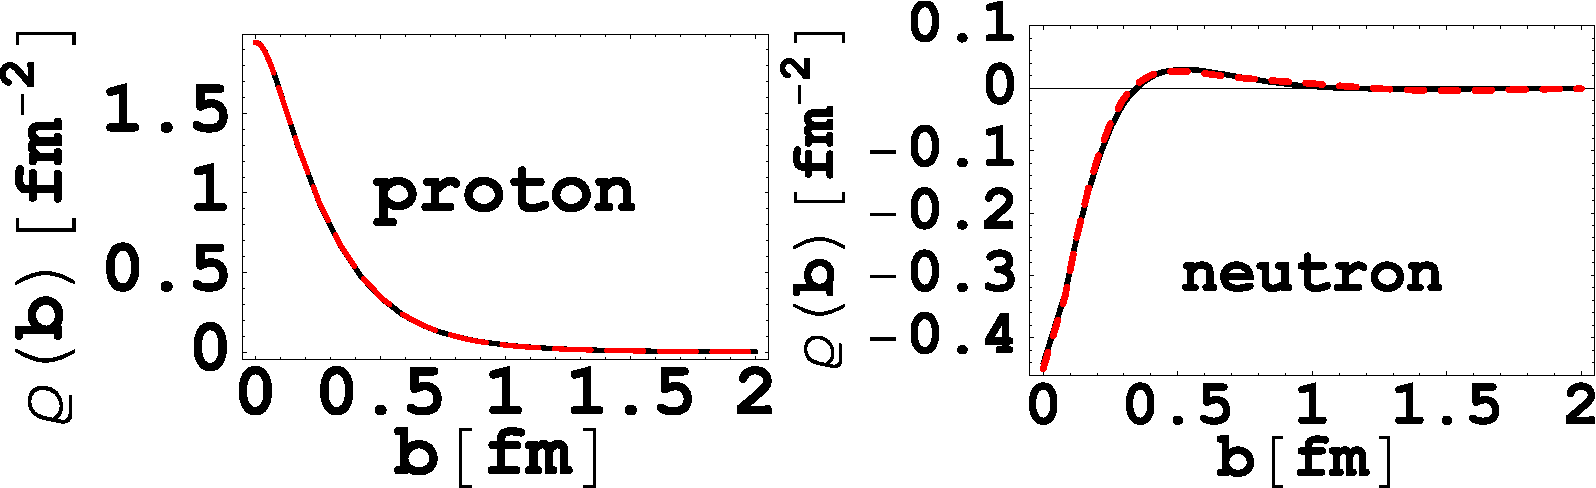
\includegraphics[width=0.9\linewidth]{charge_distribution_rotated}
    \caption{The proton charge density (left panel) and neutron charge density
	(right panel). Taken from Ref.\ \cite{miller2007}}.
    \label{fig:charge}
\end{figure}
These results further demonstrate the internal structure of the nucleon.

\section {Deep Inelastic Scattering}
\label{sec:dis}
Evidence of the point-like constituents in the nucleon first came from the deep
inelastic scattering (DIS) experiments \cite{breidenbach1969}, where a high 
energy lepton ($l$) is inelastically scattered of a nucleon ($N$), as 
illustrated in Fig.\ \ref{fig:DIS}
\begin{equation}
	l + N \rightarrow l^\prime + X.
\end{equation}
\begin{figure}[htbp!]
    \centering
    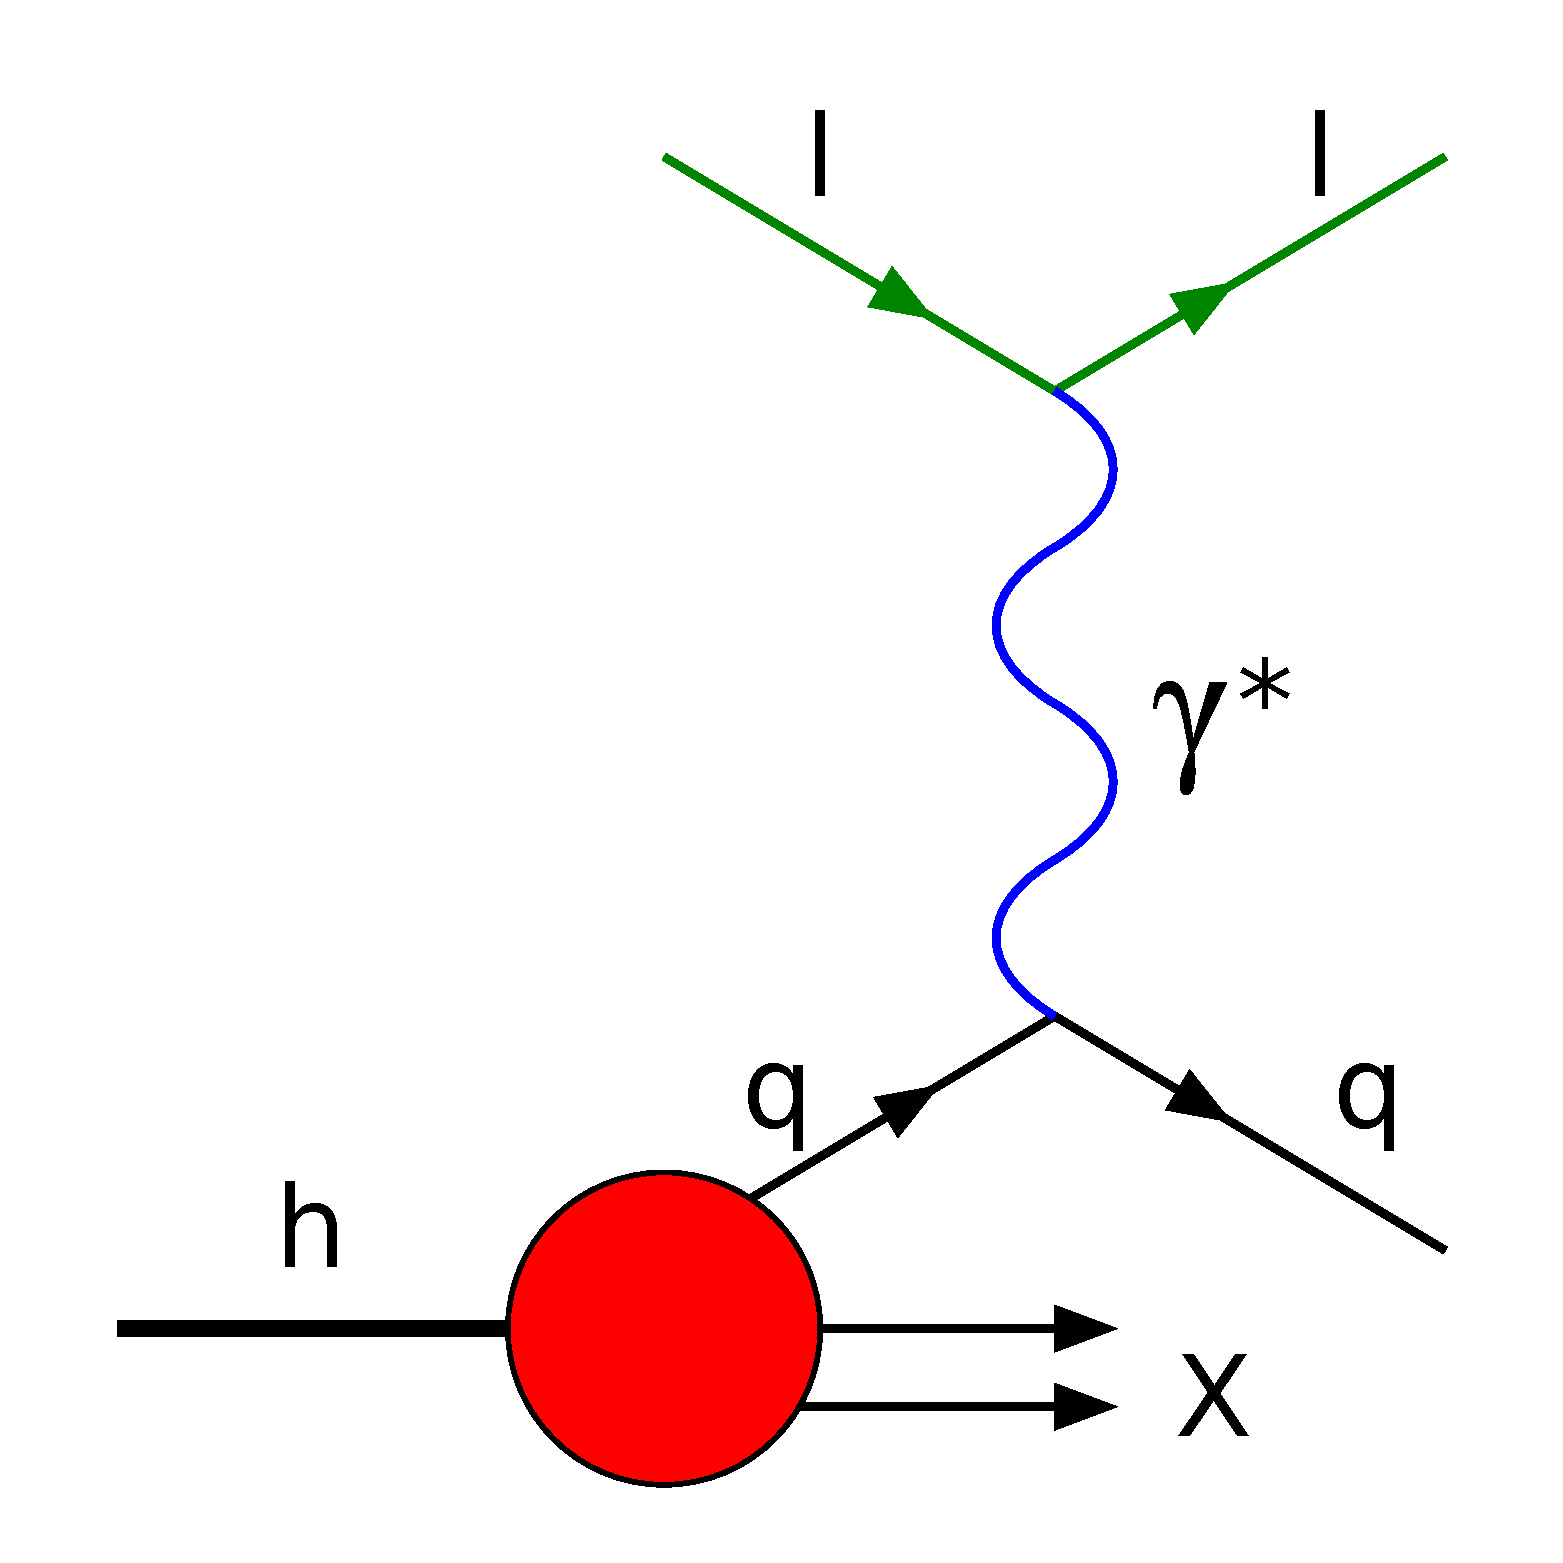
\includegraphics[width=0.3\linewidth]{DIS}
    \caption{The Feynman diagram for DIS}
    \label{fig:DIS}
\end{figure}
Similar to Eq.\ \ref{eq:ep_cs}, the DIS cross section can be expressed as 
\begin{equation}
	\eval{\frac{d^2\sigma}{dE^\prime d\Omega}}_{DIS} = \frac{\alpha^2}{4E^2 \sin^4 
	\frac{\theta}{2}} \left[ W_2\left(\nu,Q^2\right)\cos^2
	\frac{\theta}{2} + W_1\left(\nu,Q^2\right)\sin^2 \frac{\theta}{2}
	\right],
	\label{eq:DIS_cs1}
\end{equation}
where $\nu$ is the energy transferred by the scattering lepton. It is also 
customary to the define the structure functions $F_{1,2}$ from $W_{1,2}$ as:
\begin{equation}
	\begin{split}
		F_1\left(x,Q^2\right) &= MW_1\left(\nu,Q^2\right),\\
		F_2\left(x,Q^2\right) &= \nu W_2\left(\nu,Q^2\right),
	\end{split}
\end{equation}
where $x=Q^2/2M\nu$ and $M$ is the mass of the nucleon. It was observed that 
these structure functions $F_{1,2}$ are independent of $Q^2$, as illustrated in
Fig.\ \ref{fig:w2}. Fig.\ \ref{fig:w2} shows the early measurements of the 
structure function $F_2=\nu W_2$ as a function of $Q^2$ for a fixed 
$x=1/\omega=0.25$ taken from Ref.\ \cite{friedman1972}. This observation is 
known as Bjorken scaling\cite{bjorken1969}.
\begin{figure}[htpb!]
	\centering
	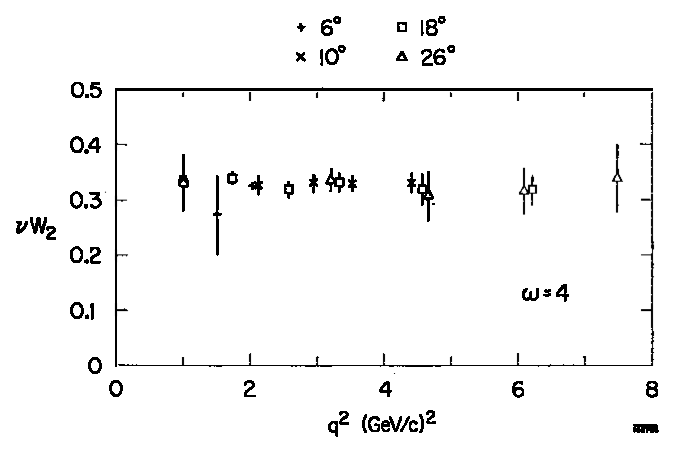
\includegraphics[width=0.5\linewidth]{nu_W2}
	\caption{Early measurement structure function $F_2=\nu W_2$ from 
	fixed-target electron–proton inelastic scattering at SLAC for 
	$x=1/\omega=0.25$ taken from Ref.\ \cite{friedman1972}. The observation 
	that $F_2(x,Q^2)$ is independent of $Q^2$ is known as Bjorken scaling. }
	\label{fig:w2}
\end{figure}

\section{Parton Model}
\label{sec:parton}
To explain the scaling behavior, Feynman proposed the parton model\cite{feynman1969}.
In this model,hadrons are treated as an extended objects which are made up of 
constituents (partons) held together by their mutual interaction. We now know 
these partons are quarks and gluons described by QCD, but this was not known at 
the time. Consider the DIS process, the hadron is Lorentz contracted in the 
direction of the collision in the center-of-mass frame, and the internal 
interaction are time dilated. Hence as the center-of-mass energy increases, the 
lifetime of the virtual partonic state is lengthened, and the time for the 
electron to pass trough the hadron is shortened. If the lifetime of the virtual
partonic states is longer than the duration of the electron-hadron interaction,
the partons are essentially frozen and the parton-parton interactions are 
neglectable. The hadrons can be considered as a collection of ``free'' partons,
and each parton may be thought of as carrying a definite fraction $x$ of the 
hadron's momentum. The high energy lepton in DIS can be treated as scattering 
of these partons elastically. The electron-parton elastic scattering can be 
calculated using perturbation QCD, where as the non-perturbation long-range 
interaction within the hadron is encapsulated in the Parton Distribution
Function (PDF) $f_{a/h}\left(x\right)$, which can be interpreted as the probability 
of finding a parton of species $a$ with fraction $x$ of the hadron's momentum. 
And the structure functions and the cross section can be written as a convolution
as non-perturbative PDF and the perturbative short range interaction. To Leading
order, the structure function $F_2\left(x\right)$ is given by
\begin{equation}
F_2\left(x\right)=x\sum_i e^2_i f_i\left(x\right),
\label{eq:F2_parton}
\end{equation}
where $e_i$ is the charge carried quark and antiquark of flavors $i$. Since, the 
gluon does not carry any charge, it does not enter the cross section at leading 
order. The ability to write the structure function and the cross section as a 
convolution of the non-perturbative PDF and pertubative short range interaction
is known as the factorization theorem \cite{collins1989}. These PDFs are also 
expected to be universal and independent of the details of the scattering 
process, as they describe the dynamics of the partons in a given hadron.

In the parton model, the structure functions $F_{1,2}$ are clearly related. And
from Eq.\ \ref{eq:DIS_cs1}, it is obvious that the structure function $F_1$ is 
related to the magnetic form factor $G_E$ in Eq.\ \ref{eq:ep_cs}. If the partons
are spin 0 particles, one would expect $F_1$ to be zero. In leading order of QCD,
only the quarks and antiquarks contribute to the cross section. Since quarks and 
antiquarks are spin 1/2 particles, this relation is given by the Callan-Gross 
relation\cite{callan1968,callan1969}
\begin{equation}
F_2\left(x\right) = 2x F_1\left(x\right).
\end{equation}
The measured deviation of the Callan-Gross relation, defined as 
\begin{equation}
K_0 = \frac{F_2}{2xF_1}-1,
\end{equation}
is shown in Fig.\ \ref{fig:callan_gross}, taken from Ref.\ \cite{kendall1991}. 
For large $Q^2$, $K_0$ is consistent with zero, establishing the parton spin as
1/2.
\begin{figure}[htbp!]
\centering
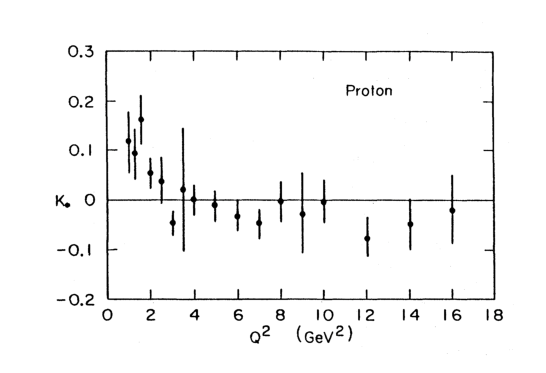
\includegraphics[width=0.5\linewidth]{Callan_Gross_relation}
\caption{The deviation from the Callan-Gross relation, defined as 
	$K_0=F_2/2xF_1 -1$, taken from Ref.\ \cite{kendall1991}. This result
	demonstrates the spin 1/2 nature of the partons.}
\label{fig:callan_gross}
\end{figure}

\section{Quantum Chromodynamics}
\label{sec:QCD}
\pdfmargincomment{General QCD}
Quantum Chromodynamics (QCD) is a theory of the strong interactions. It was 
introduced by Fritzsch and Gell-Mann \cite{fritzsch1972} and Fritzsch, Gell-Mann,
and Leutwyler \cite{fritzsch1973}. QCD is a non-abelian gauge theroy with an 
$SU(3)$ gauge symmetry applied to he color degree of freedom. The $SU(3)$ group 
chosen be to account for (a) meson states made up of $q\bar{q}$ but not $qq$ bound states.
(b) There must color singlet states. (c) The number of colors for each flavor of
must be in agreement with the measured hadronic $e^+ e^-$ cross-section.


An important feature of QCD is the asymptotic freedom. Being a renormalizable 
theory, a regularization procedure and a set of renormalization prescription 
need to be specified. In the renormalization process, the renomalized coupling $\alpha$
is introduced and this coupling would be a function of the renomalization scale $\mu$.
It is noted that the coupling constant vanishes the $Q/\mu$ tends to infinity. 
Allowing perturbative expansion of QCD at large $Q$. 


\subsection{QCD Improved Parton Model and Scaling Violation}
\label{subsec:scaling_violation}
In QCD, the parton distribution functions can be defined as matrix elements of 
operators acting on the hadron state. These operators act to count the number of
quarks and gluon carrying a fraction $\xi$ of the hadron's momentum. For quarks,
the distribution is given by\cite{collins1989} 
\begin{equation}
	f_{q/h}\left(\xi\right) = \frac{1}{4\pi}\int \dd{x} e^{-i\xi P^{+} x^{-}} \mel{P}{\bar{\psi}\left(0,x^-,0_\perp\right)\gamma^+ \mathcal{G} \psi\left(0,0,0_\perp\right)}{P},
\end{equation}
where $\mathcal{G}$ is the gauge link operator
\begin{equation}
	\mathcal{G}=\mathcal{P} \exp \left\{ ig\int_0^{x^-}\dd{y^-} A_c^+ \left(0,y^-,0_\perp\right)t_c\right\},
\end{equation}
where $\mathcal{P}$ denoted the path ordering of the gluon field operators $A_a^+$
along the path. Similarly, the gluon distribution function is given by
\begin{equation}
	f_{g/h}\left(\xi\right) = \frac{1}{2\pi\xi P^+}\int \dd{x} e^{-i\xi P^{+} x^{-}} \mel{P}{\tensor{F_a\left(0,x^-,0_\perp\right)}{^+^\nu}\gamma^{+} \tensor{\mathcal{G}}{_a_b} \tensor{F_b\left(0,0,0_\perp\right)}{_\nu^+}}{P},
\end{equation}
where $F^a_{\mu\nu}$ is the field operator and the octet representation of the $SU(3)$
generating matrices $t_c$ is used in $\mathcal{G}$.

\pdfmargincomment{QCD correction to parton model: Q2 dependence introduce by the 
	renormalization and factorization}

The QCD generalization of Eq.\ \ref{eq:F2_parton} is given 
\begin{equation}
\frac{1}{x}F_2\left(x,Q^2\right) = \sum_a \int_x^1 \frac{\dd{\xi}}{x}f_{a/h}\left(\xi,\mu\right)\frac{\xi}{x}H_{2a}\left( \frac{x}{\xi}, \frac{Q}{\mu}, \alpha_s\left(\mu\right)\right)
	+ \text{Remainder}
\end{equation}
The hard scattering coefficient $H_{2a}$ would be power series in $\alpha_s$. It
can be shown the remainder is suppress by powers of $Q$. Here the parton 
distribution also depends on the renormalization scale $\mu$. This scale 
dependency is introduce by the renomalization procedure. By requiring the cross 
section and the structure functions to be independent of the scale $\mu$,
one can show that the renormalization group equation for the distribution 
functions is
\begin{equation}
	\mu\frac{d}{d\mu}f_{a/h}\left(\xi,\mu\right)=\sum_b \int_\xi^1 \frac{\dd{\zeta}}{\zeta} P_{a/b}\left(\zeta,\alpha_s\left(\mu\right)\right) f_{b/h}\left(\frac{\xi}{\zeta},\mu\right),
\end{equation}
where $P_{a/b}$ is the Altarelli-Parisi kernel\cite{altarelli1977}. 

It is customary to choose $\mu =Q$ to avoid large logarithms of $\mu /Q$ in the 
power expansions of $H$ As such the $\mu$ dependency in the parton distribution 
functions can be interpreted as a virtual photon with higher $Q$ would probe the
nucleon with better resolution. 

\section{Sum Rules}
\label{sec:sum_rules}
Since hadrons are characterized by their quantum numbers, and these quantum numbers 
are carried by the constituent partons, these quantum numbers serve as constrains
on these PDF. For example, using the numbers of valance quarks in the protons, 
one can impose the following constrains
\begin{equation}
\begin{split}
	\int_{0}^{1} \dd{x} \left[f_{u/p} \left(x\right)-f_{\bar{u}/p} \left(x\right)\right]&=2,\\
	\int_{0}^{1} \dd{x} \left[f_{d/p} \left(x\right)-f_{\bar{d}/p} \left(x\right)\right]&=1,\\
	\int_{0}^{1} \dd{x} \left[f_{i/p} \left(x\right)-f_{\bar{i}/p} \left(x\right)\right]&=0 \qquad \text{other quark flavors}.
\end{split}
\end{equation}
And the momentum of the hadron should be distributed among the partons, hence
\begin{equation}
	\sum_{i=q,\bar{q},g}\int_{0}^{1} \dd{x} xf_{i/h}\left(x\right)=1.
\end{equation}
An important sum rule is the Gottfired sum rule\cite{gottfried1967}. It can be obtained
if we use the isospin symmetry to relate the neutron distributions to those of 
the proton, namely the (anti) up quark in the neutron would have the same distribution 
as (anti) down quark in proton, and vice-versa; the other quarks flavors and gluon
distribution would be the same in both proton and neutron. Using this relation
\begin{equation}
\begin{split}
	S_G & = \int_0^1 \frac{\dd{x}}{x}\left(F_2^{p} - F_{2}^{n}\right)\\
	    & = \frac{1}{3} \int_0^1 \dd{x} \left[u\left(x\right) - d\left(x\right) 
			+ \bar{u}\left(x\right) - \bar{s}\left(x\right)\right]\\
		& = \frac{1}{3} \int_0^1 \dd{x} \left[u\left(x\right) - \bar{u}\left(x\right)\right]
			- \frac{1}{3} \int_0^1 \dd{x} \left[d\left(x\right) - \bar{d}\left(x\right)\right]
			+ \frac{2}{3} \int_0^1 \dd{x} \left[\bar{u}\left(x\right)-\bar{d}\left(x\right)\right]\\
		& = \frac{1}{3} + \frac{2}{3} \int_0^1 \dd{x} \left[\bar{u}\left(x\right)-\bar{d}\left(x\right)\right]. 
\end{split}
\end{equation}
If one made the naive assumption that $\int_0^1\dd{x} \bar{u}\left(x\right)=\int_0^1\dd{x} \bar{d}\left(x\right)$,
then $S_G$ would be expected to be $1/3$. And this assumption can be tested using DIS.
One of the early measurements is from the New Muon Collaboration (NMC)\cite{amaudruz1991}. 
The measured $F_2^p-F_2^n$ by NMC is shown in Fig.\ \ref{fig:NMC_Gottfried}. 
\begin{figure}[htbp!]
	\centering
	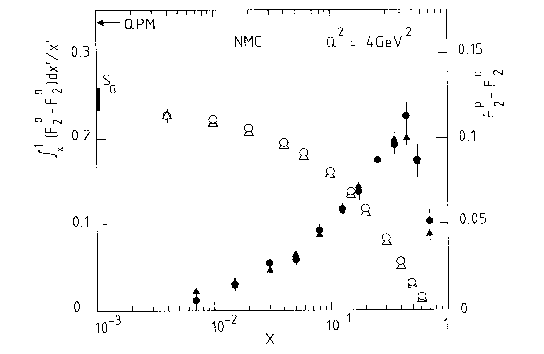
\includegraphics[width=0.7\linewidth]{Gottfried}
	\caption{The difference $F_2^p -F_2^n$ (solid and scale to the right) and 
		$\int_{x_{min}}^1 (F_2^p-F_2^n)\dd{x}/x$ (open and scale to the left) 
		determined by NMC, taken from Ref.\ \cite{amaudruz1991}. The extrpolation
		to $x_{min}=0$ is indicated by the bar.}
	\label{fig:NMC_Gottfried}
\end{figure}
The measured Gottfried sum is $0.240 \pm 0.016$, which is significantly below 
$1/3$, suggesting an asymmetry in the light sea-quarks.


\section{Drell-Yan Process}
\label{sec:DY}
Another process for probing the hadron structure is the Drell-Yan process\cite{drell1970}.
As illustrated in Fig.\ \ref{fig:DY}, this process involves two partons from the 
two colliding hadrons to annihilate and form a lepton pair.
\begin{equation}
	h_A + h_B \rightarrow l + \bar{l} + X.
\end{equation}
The Drell-Yan process is related to the DIS process via crossing symmetry.
\begin{figure}[htbp!]
	\centering
	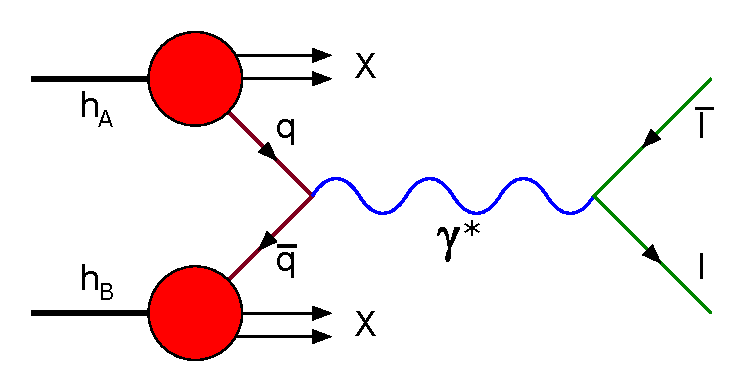
\includegraphics[width=0.5\linewidth]{Drell-Yan}
    \caption{The Feynman diagram for the Drell-Yan process}
    \label{fig:DY}
\end{figure}
Similar to DIS, the Drell-Yan cross section can be factorized into the non-perturbative
PDF and the purtabative parton-parton scattering. And the proof of factorization 
theorem for Drell-Yan can be found in Ref.\ \cite{collins1989}. At leading-order 
of QCD, the cross section can be written as
\begin{equation}
	\frac{d^2\sigma_{DY}}{dx_{1}dx_{2}} = \frac{4\pi\alpha^2}{9M^2}\sum_i e^2_i
		\left[f_{i/A}\left(x_1\right)f_{\bar{i}/B}\left(x_2\right) +
			f_{\bar{i}/A}\left(x_1\right)f_{i/B}\left(x_2\right)
		\right].
	\label{eq:DY_cs}
\end{equation}
Fig.\ \ref{fig:scaling} shows some of the existing data on DIS and Drell-Yan. By
performing a global fit to both DIS and Drell-Yan data, the parton distribution 
functions can be extracted. The ability to fit both DIS and Drell-Yan data using 
the same PDF demonstrate the universality of the PDF and the usefulness of the 
factorization theorem. 
\pdfmargincomment{factorization and universality of PDF, scaling plot for both DIS 
	and DY.May need better plot. Shows some PDF extraction}
\begin{figure}[htbp!]
	\centering
	\begin{subfigure}{0.45\linewidth}
		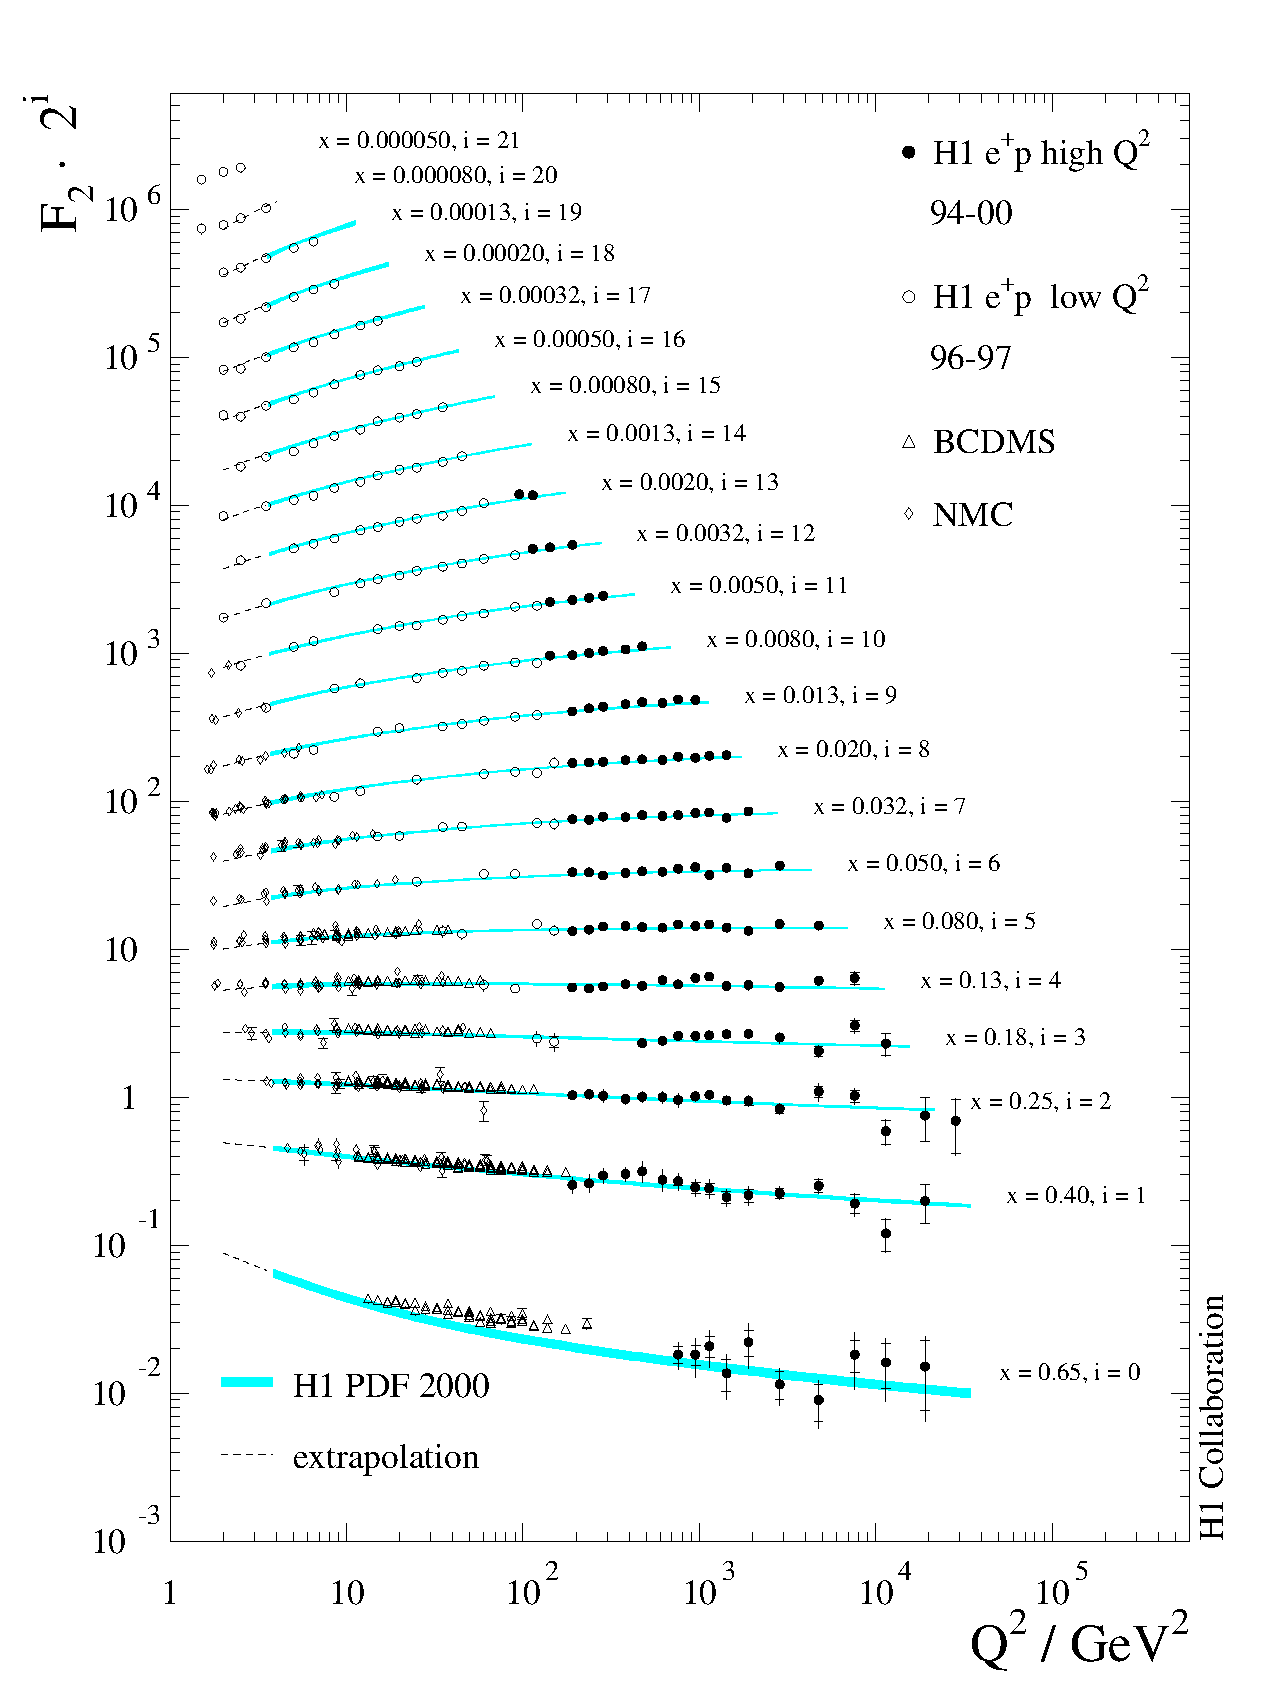
\includegraphics[width=\linewidth]{DIS_scaling}
		\caption{taken from Ref.\ \cite{theh1collaboration2003}}
		\label{subfig:DIS_scaling}
	\end{subfigure}
	\begin{subfigure}{0.45\linewidth}
		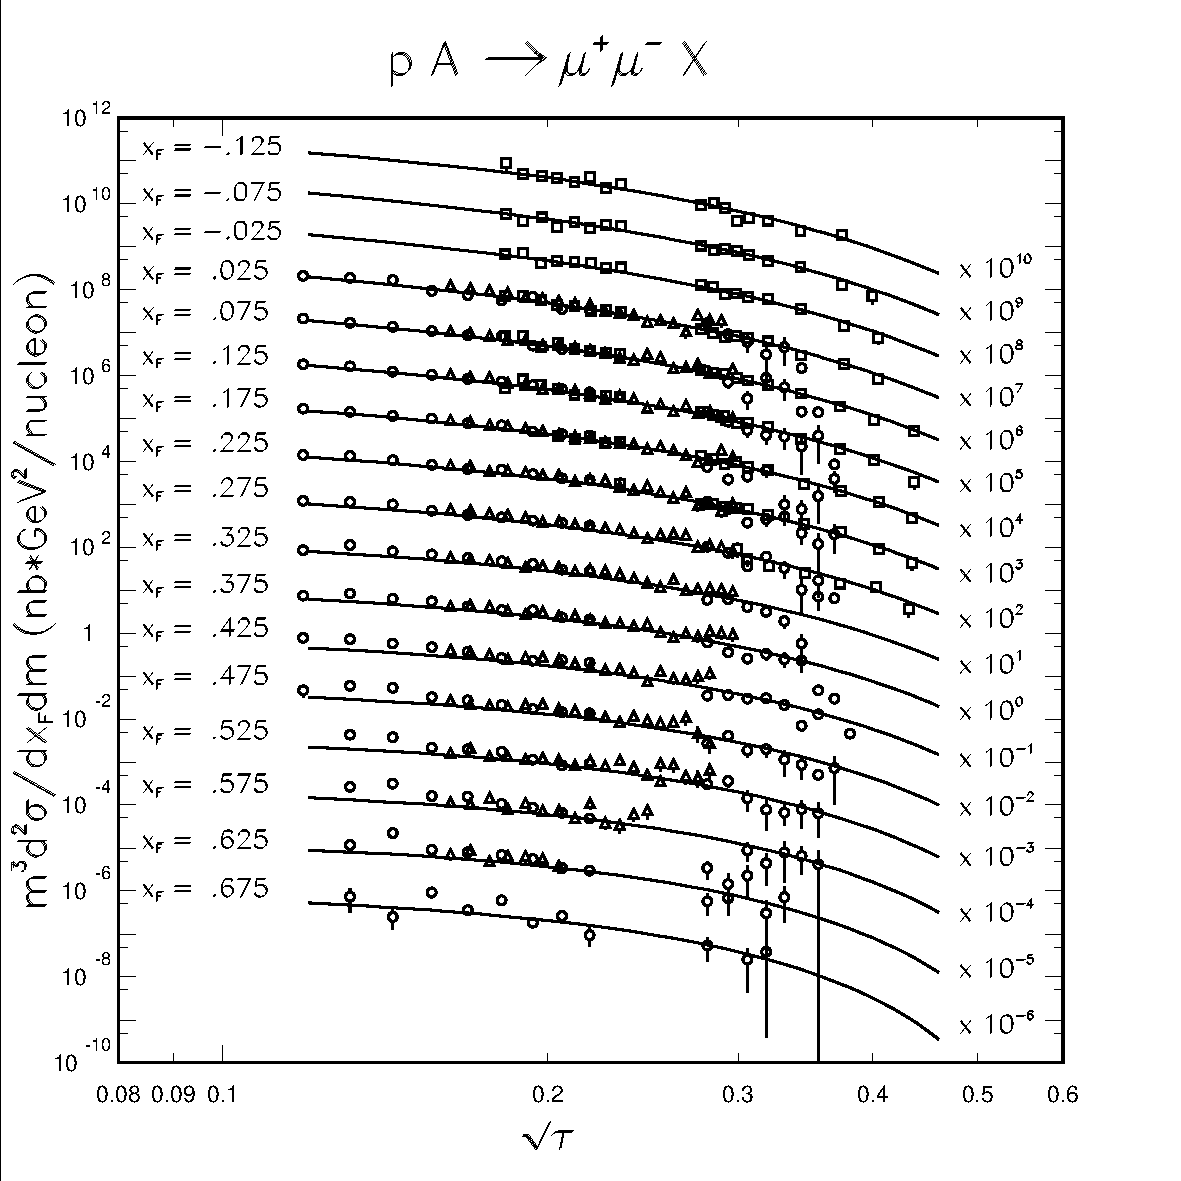
\includegraphics[width=\linewidth]{DY_scaling}
		\caption{taken from Ref.\ \cite{mcgaughey1999}}
		\label{subfig:DY_scaling}
	\end{subfigure}
	\caption{Compilation of data on DIS (\subref{subfig:DIS_scaling}) and 
		Drell-Yan (\subref{subfig:DY_scaling})}
	\label{fig:scaling}
\end{figure}
One of the advantages of Drell-Yan over DIS is the explicit separation of the quark
and anti-quark distributions in Eq.\ \ref{eq:DY_cs}. At large $x$, DIS cross section 
is dominated by the valance quark distribution. On the other hand, in the region $x_1 \gg x_2$,
the valance quark in the Drell-Yan process is more likely to come from the beam 
hadron, and the anti-quark is more likely to come from the target hadron. Hence,
Drell-Yan can be more sensitive to the anti-quark distribution than DIS. In 
particular, for high $x_F$ and using the fact there are two up valance quarks in 
protons, the $(p+d/2(p+p))$ Drell-Yan cross section ratio can be approximated as 
\begin{equation}
	\frac{\sigma^{p+d}}{2\sigma^{p+p}} \approx \frac{1}{2} \left( 1+ \frac{\bar{d}\left(x_2\right)}{\bar{u}\left(x_2\right)} \right).
\end{equation}
Thus the Drell-Yan process has been used in many experiments to probe the sea-quarks 
asymmetry.


\subsection{E866/NuSea}
\label{sec:E866}
The E866/NuSea experiment was designed to measure the flavor structure of the sea 
quark over a broad range of $x$ to higher precision than previous experiments. The 
experiment utilized the \SI{800}{\GeV} proton beam from the Tevatron on liquid 
hydrogen and deuterium targets. The measured deuterium over hydrogen cross section 
ratio from E866/NuSea is shown in Fig.\ \ref{fig:e866_result}. They observed the
cross section ratio drop off below unity at $x_2>0.25$, suggesting the $\bar{d}/\bar{u}$ 
ratio drop off below 1. Various models had difficulties explaining this surprising 
behavior. Due to the large uncertainty on the data points at large $x_2$, a new 
experiment was needed to explore sea quark asymmetry the high $x$ region with better 
accuracy.
\begin{figure}[htbp!]
	\centering
	\begin{subfigure}{0.45\linewidth}
		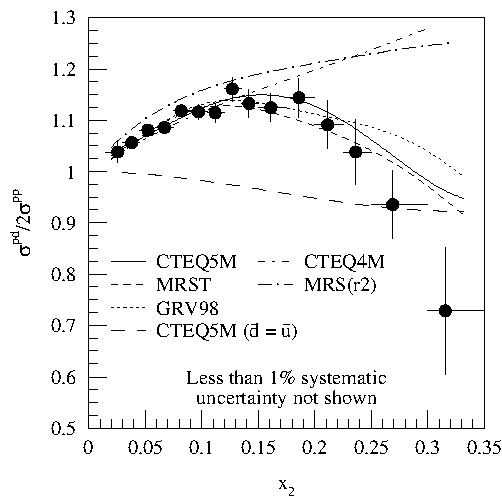
\includegraphics[width=\linewidth]{e866_csr}
		\caption{$(p+p)/2(p+d)$ Drell-Yan cross section ratio}
		\label{subfig:e866_csr}
	\end{subfigure}
	\begin{subfigure}{0.45\linewidth}
		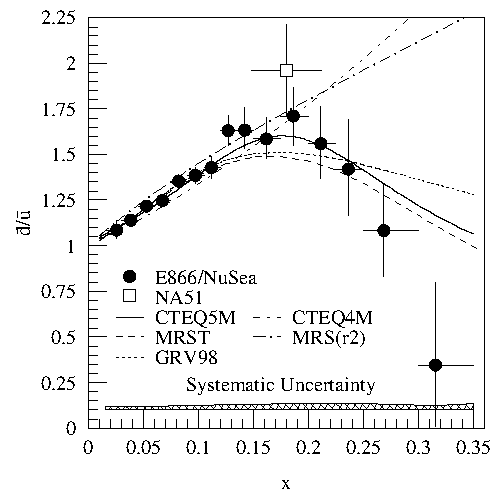
\includegraphics[width=\linewidth]{e866_dbarubar}
		\caption{$\bar{d}/\bar{u}$ extracted from E866 result.}
		\label{subfig:e866_dbarubar}
	\end{subfigure}
	\caption{The E866 result taken from Ref.\ \cite{towell2001}}
	\label{fig:e866_result}
\end{figure}



\section{Charmonium Production}
\label{sec:jpsi}
Yet another process for probing the nucleon structure is via the charmonium production\cite{peng1995,chang2020}.
Unlike DIS and Drell-Yan, the charmonium production involves the strong interaction
at leading-order. Therefore it can be used to probe the gluon structure, which is 
less sensitive in DIS or Drell-Yan, and the quark anti-quark structure. However, 
because of the non-pertiubative nature of QCD, there are various models for 
calculating the charmonium production. The models usually separate the production
mechanism into two parts, the production of heavy-quark pairs and the subsequent
hadronization into quarkonium states. One of the early approaches is the Color 
Evaporation method (CEM)\cite{einhorn1975,bodwin1995,bodwin1997}. The heavy-quark 
pairs production is expanded in terms of the strong coupling constant $\alpha_s$
and is calculated with perturbative QCD (pQCD). CEM then assumes a constant 
probability $F$ for the $c\bar{c}$ pairs to hadronize into different charmonium
state and this probability is independent of the kinematics or the production
subprocess. The charmonium production cross section in the CEM framework can be 
expressed as
\begin{equation}
    \begin{split}
        \left.\frac{d\sigma}{dx_F}\right|_{J/\Psi} &= F \sum_{i,j = q,\bar{q},G}\int^{2m_D}_{2m_c} dM_{c\bar{c}}  \frac{2M_{c\bar{c}}}{s\sqrt{x_F^2+4M_{c\bar{c}}^2/s}}\\
        &\cross f_{i/A}\left(x_1,\mu_F\right)f_{j/B}\left(x_2,\mu_F\right)\sigma\left[ij\rightarrow c\bar{c}X\right]\left(x_1P_A,x_2P_B,\mu_F,\mu_R \right),
    \end{split}
\end{equation}
where $i$,$j$ denote the type of interacting partons. At leading-order, the 
$c\bar{c}$ pairs are produced via two subprocesses, gluon fusion and 
quark-antiquark annihilation, as illustrated in Fig.\ \ref{fig:charmonium}.
\begin{figure}[htpb!]
    \centering
    \begin{subfigure}{0.4\linewidth}
        \begin{subfigure}{\linewidth}
        \begin{tikzpicture}
 \tikzstyle{every node}=[font=\large]
    \begin{feynman}
    \vertex  (a1);
    \vertex [right= of a1, blob] (a2) {};
    \vertex [right= 4cm of a2] (a3) ;
    \vertex [below= 2cm of a1] (b1);
    \vertex [below= 2cm of a2,blob] (b2) {};
    \vertex[below= 2cm of a3] (b3);
    \vertex  at ($(b2) + (1.5cm , +1cm)$) [dot] (d);
    \vertex [right= 1cm of d] (d1);
     \vertex at ($(d1) + (1.5cm , +0.7cm)$) (c1) {$c$};
     \vertex at ($(d1) + (1.5cm , -0.7cm)$) (c2) {$\bar{c}$};
     \diagram*{
     (a1) --[fermion](a2),
     (a2) --[double](a3),
     (b1) --[fermion](b2),
     (b2) --[double](b3),
     (b2) --[gluon, edge label'=\(g\)] (d),
     (a2) --[gluon, edge label=\(g\)](d),
     (d) --[gluon](d1),
     (c2) --[fermion] (d1);
     (d1) --[fermion] (c1);
     };
    \end{feynman}
\end{tikzpicture}
        \end{subfigure}
        \begin{subfigure}{\linewidth}
        \begin{tikzpicture}
\tikzstyle{every node}=[font=\large]
    \begin{feynman}
    \vertex  (a1);
    \vertex [right= of a1, blob] (a2) {};
    \vertex [right= 4cm of a2] (a3) ;
    \vertex [below= 2cm of a1] (b1);
    \vertex [below= 2cm of a2,blob] (b2) {};
    \vertex [below= 2cm of a3] (b3);
    \vertex  at ($(b2) + (1.5cm , +0.666cm)$) [dot] (d);
    \vertex [above= 0.668cm of d] (d1);
     \vertex [right= 2.25cm of d1] (c1) {$c$};
     \vertex [right= 2.25cm of d] (c2) {$\bar{c}$};
     \diagram*{
     (a1) --[fermion](a2),
     (a2) --[double](a3),
     (b1) --[fermion](b2),
     (b2) --[double](b3),
     (b2) --[gluon, edge label=$g$] (d),
     
     (a2) --[gluon, edge label'=$g$](d1),
     (d) --[fermion](d1),
     (d1) --[fermion] (c1);
     (c2) --[fermion] (d);
     };
    \end{feynman}
\end{tikzpicture}
        \end{subfigure}
        \caption{gluon fusion\label{subfig:gluon}}
    \end{subfigure}
    \quad
    \begin{subfigure}{0.4\linewidth}
    \begin{tikzpicture}
\tikzstyle{every node}=[font=\large]
    \begin{feynman}
    \vertex  (a1);
    \vertex [right= of a1, blob] (a2) {};
    \vertex [right= 4cm of a2] (a3) ;
    \vertex [below= 2cm of a1] (b1);
    \vertex [below= 2cm of a2,blob] (b2) {};
    \vertex[below= 2cm of a3] (b3);
    \vertex  at ($(b2) + (1.5cm , +1cm)$) [dot] (d);
    \vertex [right= 1 cm of d] (d1);
     \vertex at ($(d1) + (1.5cm , +0.7cm)$) (c1) {$c$};
     \vertex at ($(d1) + (1.5cm , -0.7cm)$) (c2) {$\bar{c}$};
     \diagram*{
     (a1) --[fermion](a2),
     (a2) --[double](a3),
     (b1) --[fermion](b2),
     (b2) --[double](b3),
     (d) --[fermion, edge label=$\bar{q}$] (b2),
     (a2) --[fermion, edge label=$q$](d),
     (d) --[gluon](d1),
     (c2) --[fermion] (d1);
     (d1) --[fermion] (c1);
     };
    \end{feynman}
\end{tikzpicture}
    \caption{quark-antiquark annihilation\label{subfig:qqbar}}
    \end{subfigure}
    \caption{The Feynman diagram for $c\bar{c}$ pair production}
    \label{fig:charmonium}
\end{figure}
The calculated cross section for $J/\Psi$ production in $p+p$ at 120 GeV using 
CEM is shown in Fig.\ \ref{fig:cem_cs}. The relative importance of gluon fusion 
and quark-antiquark annihilation is a strong function of $x_F=2P_L/\sqrt{s}$, 
where $P_L$ is the longitudinal momentum of the $J/\Psi$ meson in the 
hadron-hadron center-of-mass frame and $\sqrt{s}$ is the total energy in this 
frame. At large $x_F$, the quark-antiquark annihilation is the dominant subprocess.  
\begin{figure}[h!]
    \centering
    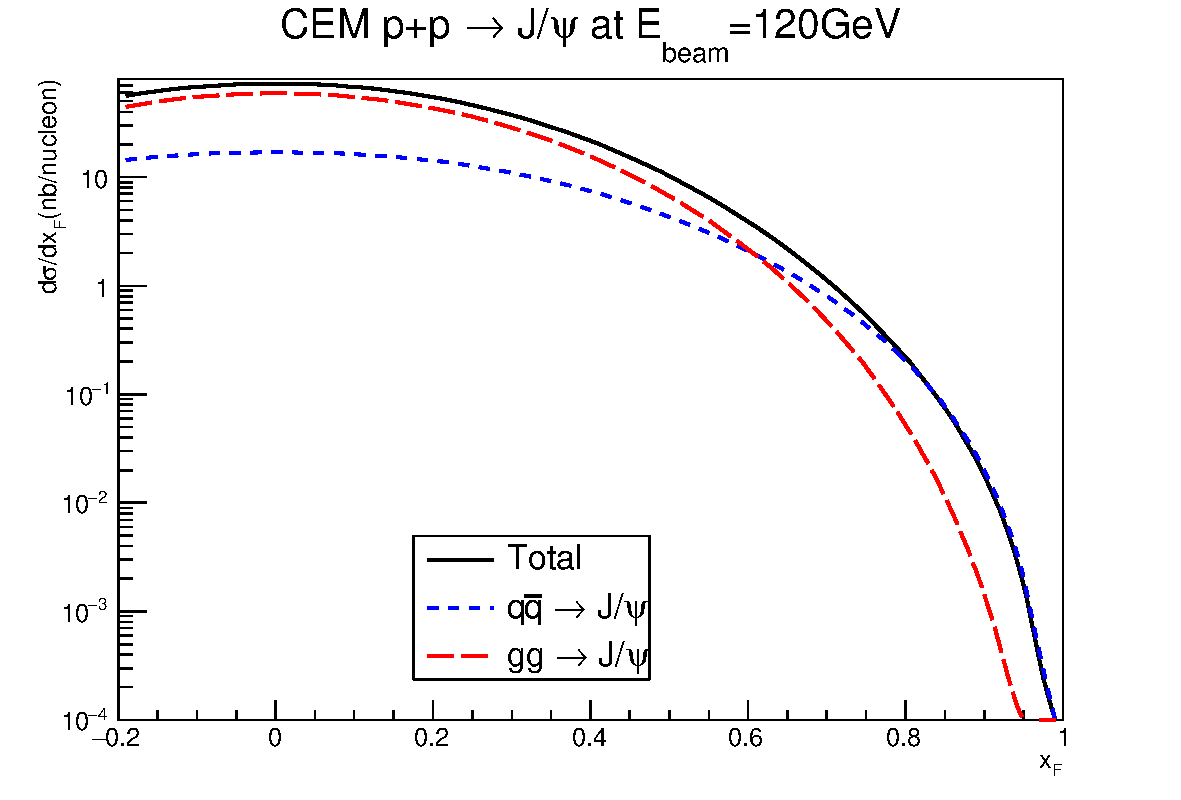
\includegraphics[width=0.45\linewidth]{pp_norm_cs_NLO_pp}
    \caption{Calculated cross section for $J/\Psi$ production using CEM model. 
		The CEM code is obtained from Ref.\ \cite{mangano1993}.}
    \label{fig:cem_cs}
\end{figure}

Another theoretical model for quarkonium productions is the non-relativistic 
QCD (NRQCD) \cite{bodwin1995,bodwin1997}. Unlike CEM, the probability of 
hadronization depends on the color and spin state of the $c\bar{c}$ pairs and 
is described by various long-distance matrix elements (LDMEs). The quarkonium 
production cross section in this framework is given as
\begin{equation}
    \begin{split}
        \frac{d\sigma^H}{dx_F} &=\sum_{i,j = q,\bar{q},G}\int^1_0 dx_1 dx_2 \delta(x_F-x_1+x_2)\\
        &\cross f_{i/A}\left(x_1,\mu_F\right)f_{j/B}\left(x_2,\mu_F\right)\hat{\sigma}\left[ij\rightarrow H\right]\left(x_1P_A,x_2P_B,\mu_F,\mu_R , m_c\right),
    \end{split}
\end{equation}
\begin{equation}
    \hat{\sigma}\left[ij\rightarrow H\right]= \sum_n C^{ij}_{c\bar{c}\left[n\right]}\left(x_1P_A,x_2P_B,\mu_F,\mu_R , m_c\right)\expval{O^H_n \left[^{2S+1}L_J\right]},
\end{equation}
where the $c\bar{c}$ pair is labeled by its color ($n$), spin ($S$), orbital 
angular momentum ($L$) and total angular momentum ($J$). The coefficient 
$C^{ij}_{c\bar{c}\left[n\right]}$ describes the production of $c\bar{c}$ pair 
with specific color-spin state and is calculated perturbatively in powers of 
$\alpha_s$ using pQCD. The LDME $\expval{O^H_n \left[^{2S+1}L_J\right]}$ accounts 
for the hardronization probability for a specfic $c\bar{c}$ state into the 
charmonium state $H$. These LDMEs are obtained by fitting to data and assumed to
be universal, independent of beam or target hadrons and the energy scale. The 
calculated cross sections for $J/\Psi$ and $\Psi'$ production using NRQCD for 
$p+p$ at 120 GeV are shown in Fig.\ \ref{fig:NRQCD_cs}. In this model, quark-antiquark
annihilation is more important than suggested by CEM. This model also suggests 
that the relative importance of the two subprocess depends on the charmonium state. 
In particular, Fig.\ \ref{fig:NRQCD_cs} shows that the quark-antiquark annihilation 
is the dominatent process for $\Psi^\prime$ production.
\begin{figure}[h!]
    \centering
    \begin{subfigure}{0.45\linewidth}
    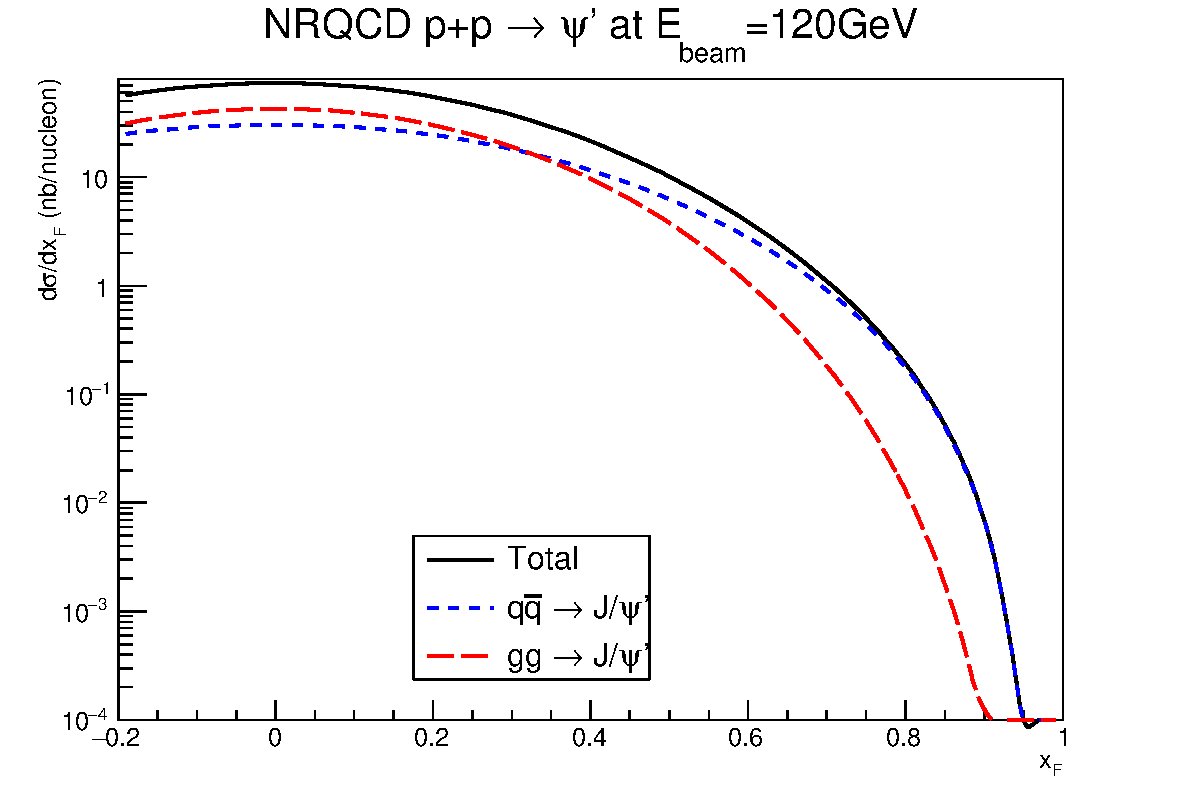
\includegraphics[width=\linewidth]{jpsi_cs_pp}
    \caption{$J/\Psi$ production}
    \end{subfigure}
    \quad
    \begin{subfigure}{0.45\linewidth}
    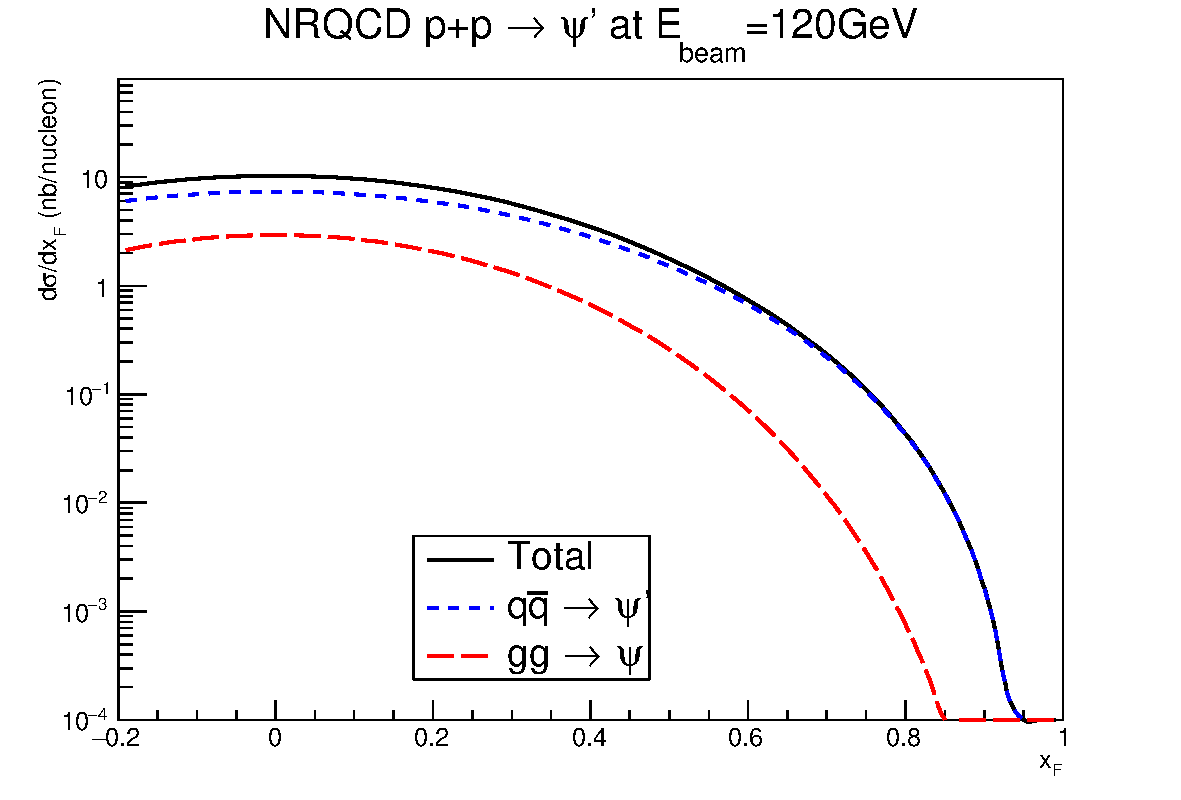
\includegraphics[width=\linewidth]{psip_cs_pp}
    \caption{$\Psi'$ production}
    \end{subfigure}
    \caption{Calculated cross section for charmonium production using NRQCD model
		\cite{chang2021}. CT14nlo is used as the proton PDF. The LDMEs used are
		taken from table \num{4} in Ref.\ \cite{hsieh2021}, and are obtained from a 
		global fit to fixed-target charmonium production data. }
    \label{fig:NRQCD_cs}
\end{figure}

\pdfmargincomment{what is physical significant of the nuclear dependence}

\ifSubfilesClassLoaded{ \printbibliography[heading=bibintoc,title={References}]}{}

\end{document}
